% Created by tikzDevice version 0.12.6 on 2025-08-19 18:43:27
% !TEX encoding = UTF-8 Unicode
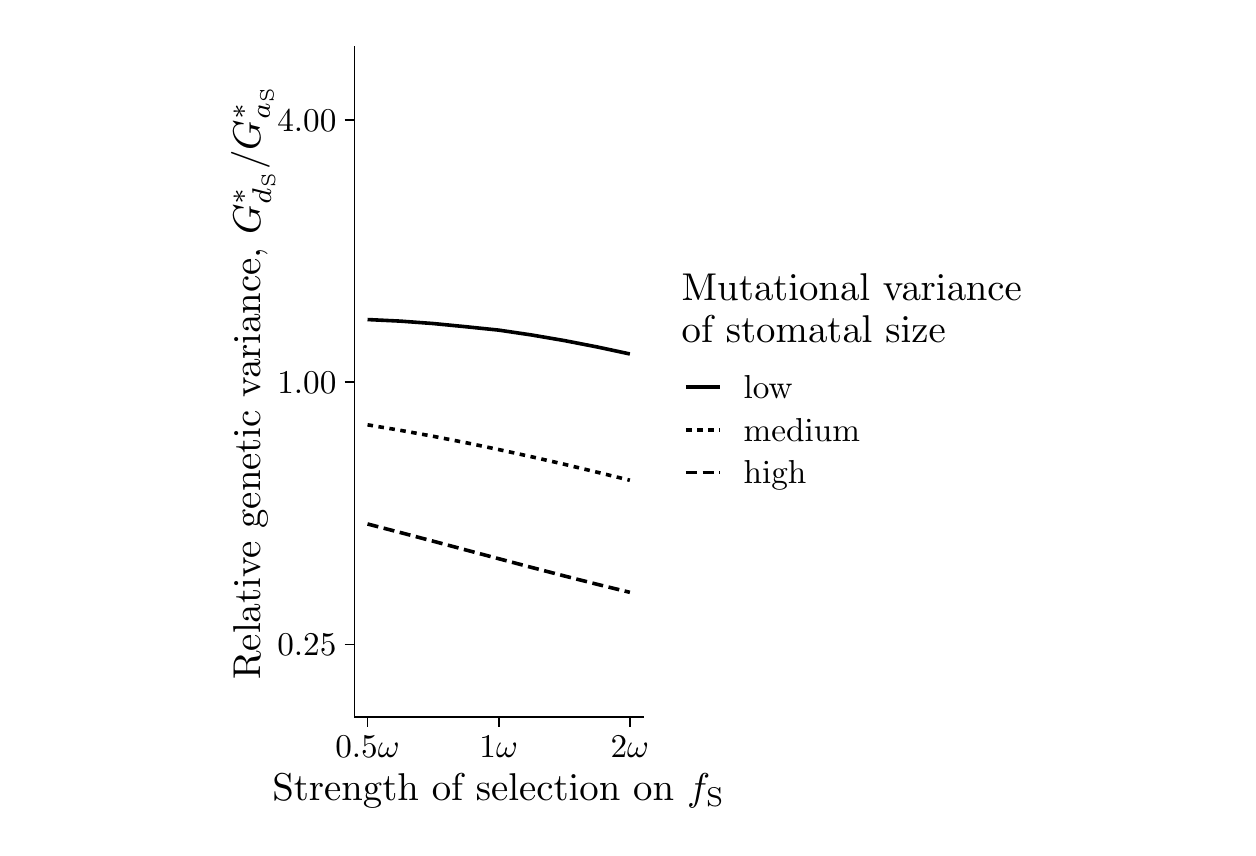
\begin{tikzpicture}[x=1pt,y=1pt]
\definecolor{fillColor}{RGB}{255,255,255}
\path[use as bounding box,fill=fillColor,fill opacity=0.00] (0,0) rectangle (433.62,289.08);
\begin{scope}
\path[clip] (118.07, 39.96) rectangle (222.34,282.08);
\definecolor{drawColor}{RGB}{0,0,0}

\path[draw=drawColor,line width= 1.3pt,line join=round] (122.81,183.61) --
	(134.66,183.04) --
	(146.51,182.17) --
	(158.36,181.01) --
	(170.21,179.79) --
	(182.06,178.04) --
	(193.91,176.01) --
	(205.76,173.71) --
	(217.60,171.17);

\path[draw=drawColor,line width= 1.3pt,dash pattern=on 2pt off 2pt ,line join=round] (122.81,145.57) --
	(134.66,143.58) --
	(146.51,141.43) --
	(158.36,139.11) --
	(170.21,136.63) --
	(182.06,134.03) --
	(193.91,131.31) --
	(205.76,128.45) --
	(217.60,125.54);

\path[draw=drawColor,line width= 1.3pt,dash pattern=on 4pt off 2pt ,line join=round] (122.81,109.74) --
	(134.66,106.65) --
	(146.51,103.52) --
	(158.36,100.35) --
	(170.21, 97.19) --
	(182.06, 94.05) --
	(193.91, 90.96) --
	(205.76, 87.95) --
	(217.60, 85.04);
\end{scope}
\begin{scope}
\path[clip] (  0.00,  0.00) rectangle (433.62,289.08);
\definecolor{drawColor}{RGB}{0,0,0}

\path[draw=drawColor,line width= 0.6pt,line join=round,line cap=rect] (118.07, 39.96) --
	(118.07,282.08);
\end{scope}
\begin{scope}
\path[clip] (  0.00,  0.00) rectangle (433.62,289.08);
\definecolor{drawColor}{RGB}{0,0,0}

\node[text=drawColor,anchor=base east,inner sep=0pt, outer sep=0pt, scale=  1.20] at (111.57, 62.09) {0.25};

\node[text=drawColor,anchor=base east,inner sep=0pt, outer sep=0pt, scale=  1.20] at (111.57,156.89) {1.00};

\node[text=drawColor,anchor=base east,inner sep=0pt, outer sep=0pt, scale=  1.20] at (111.57,251.68) {4.00};
\end{scope}
\begin{scope}
\path[clip] (  0.00,  0.00) rectangle (433.62,289.08);
\definecolor{drawColor}{RGB}{0,0,0}

\path[draw=drawColor,line width= 0.6pt,line join=round] (114.57, 66.23) --
	(118.07, 66.23);

\path[draw=drawColor,line width= 0.6pt,line join=round] (114.57,161.02) --
	(118.07,161.02);

\path[draw=drawColor,line width= 0.6pt,line join=round] (114.57,255.82) --
	(118.07,255.82);
\end{scope}
\begin{scope}
\path[clip] (  0.00,  0.00) rectangle (433.62,289.08);
\definecolor{drawColor}{RGB}{0,0,0}

\path[draw=drawColor,line width= 0.6pt,line join=round,line cap=rect] (118.07, 39.96) --
	(222.34, 39.96);
\end{scope}
\begin{scope}
\path[clip] (  0.00,  0.00) rectangle (433.62,289.08);
\definecolor{drawColor}{RGB}{0,0,0}

\path[draw=drawColor,line width= 0.6pt,line join=round] (122.81, 36.46) --
	(122.81, 39.96);

\path[draw=drawColor,line width= 0.6pt,line join=round] (170.21, 36.46) --
	(170.21, 39.96);

\path[draw=drawColor,line width= 0.6pt,line join=round] (217.60, 36.46) --
	(217.60, 39.96);
\end{scope}
\begin{scope}
\path[clip] (  0.00,  0.00) rectangle (433.62,289.08);
\definecolor{drawColor}{RGB}{0,0,0}

\node[text=drawColor,anchor=base,inner sep=0pt, outer sep=0pt, scale=  1.20] at (122.81, 25.20) {$0.5\omega$};

\node[text=drawColor,anchor=base,inner sep=0pt, outer sep=0pt, scale=  1.20] at (170.21, 25.20) {$1\omega$};

\node[text=drawColor,anchor=base,inner sep=0pt, outer sep=0pt, scale=  1.20] at (217.60, 25.20) {$2\omega$};
\end{scope}
\begin{scope}
\path[clip] (  0.00,  0.00) rectangle (433.62,289.08);
\definecolor{drawColor}{RGB}{0,0,0}

\node[text=drawColor,anchor=base,inner sep=0pt, outer sep=0pt, scale=  1.40] at (170.21,  9.72) {Strength of selection on $f_\mathrm{S}$};
\end{scope}
\begin{scope}
\path[clip] (  0.00,  0.00) rectangle (433.62,289.08);
\definecolor{drawColor}{RGB}{0,0,0}

\node[text=drawColor,rotate= 90.00,anchor=base,inner sep=0pt, outer sep=0pt, scale=  1.40] at ( 84.02,161.02) {Relative genetic variance, $G^*_{d_\mathrm{S}} / G^*_{a_\mathrm{S}}$};
\end{scope}
\begin{scope}
\path[clip] (  0.00,  0.00) rectangle (433.62,289.08);
\definecolor{drawColor}{RGB}{0,0,0}

\node[text=drawColor,anchor=base west,inner sep=0pt, outer sep=0pt, scale=  1.40] at (236.34,190.36) {Mutational variance};

\node[text=drawColor,anchor=base west,inner sep=0pt, outer sep=0pt, scale=  1.40] at (236.34,175.24) {of stomatal size};
\end{scope}
\begin{scope}
\path[clip] (  0.00,  0.00) rectangle (433.62,289.08);
\definecolor{drawColor}{RGB}{0,0,0}

\path[draw=drawColor,line width= 1.3pt,line join=round] (237.88,159.18) -- (250.20,159.18);
\end{scope}
\begin{scope}
\path[clip] (  0.00,  0.00) rectangle (433.62,289.08);
\definecolor{drawColor}{RGB}{0,0,0}

\path[draw=drawColor,line width= 1.3pt,dash pattern=on 2pt off 2pt ,line join=round] (237.88,143.78) -- (250.20,143.78);
\end{scope}
\begin{scope}
\path[clip] (  0.00,  0.00) rectangle (433.62,289.08);
\definecolor{drawColor}{RGB}{0,0,0}

\path[draw=drawColor,line width= 1.3pt,dash pattern=on 4pt off 2pt ,line join=round] (237.88,128.38) -- (250.20,128.38);
\end{scope}
\begin{scope}
\path[clip] (  0.00,  0.00) rectangle (433.62,289.08);
\definecolor{drawColor}{RGB}{0,0,0}

\node[text=drawColor,anchor=base west,inner sep=0pt, outer sep=0pt, scale=  1.20] at (258.74,155.05) {low};
\end{scope}
\begin{scope}
\path[clip] (  0.00,  0.00) rectangle (433.62,289.08);
\definecolor{drawColor}{RGB}{0,0,0}

\node[text=drawColor,anchor=base west,inner sep=0pt, outer sep=0pt, scale=  1.20] at (258.74,139.65) {medium};
\end{scope}
\begin{scope}
\path[clip] (  0.00,  0.00) rectangle (433.62,289.08);
\definecolor{drawColor}{RGB}{0,0,0}

\node[text=drawColor,anchor=base west,inner sep=0pt, outer sep=0pt, scale=  1.20] at (258.74,124.25) {high};
\end{scope}
\end{tikzpicture}
